%! Author = Len Washington III
%! Date = 9/17/2023

% Preamble
\documentclass[12pt]{report}

% Packages
\usepackage[9]{cs430lecture}

% Document
\begin{document}

%<*Lecture-Activity-9>
\section{Opening Questions}\label{sec:opening-questions-9}
\definecolor{recgreen}{HTML}{008a87}
\begin{enumerate}[label=\arabic*.]
    \item Order Statistics: Select the $i$th smallest of $n$ elements (the element with rank $i$)
	\begin{itemize}
		\item $i=1$: minimum; \answer{$1^{\mbox{st}}$ order statistic, $O(n)$}
		\item $i=n$: maximum; \answer{$n^{\mbox{st}}$ order statistic, $O(n)$}
		\item $i=\lfloor \frac{n+1}{2} \rfloor$ or $\lceil \frac{n+1}{2} \rceil$: median   \answer{Sort: $O(n\lg n)$, then take $A\left[ \frac{n}{2} \right]$ for the median, $O(1)$}
	\end{itemize}
\end{enumerate}
How fast can we solve the problem for various $i$ values?

\section{Randomized Algorithm for finding the $i$th Element}\label{sec:randomized-algorithm-for-finding-the-ith-element}
\begin{enumerate}[label=\arabic*.]
    \item Think about partition (with a random choice of the pivot\answer{``median of 3''}) from quicksort. Can you think of a way to use that and comparing the final location of the pivot to $i$, and then divide and conquer?
	\begin{figure}[H]
		\centering
		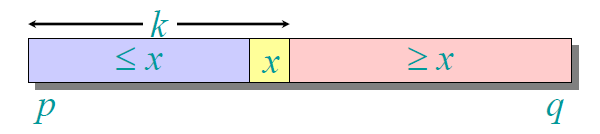
\includegraphics[width=\textwidth]{9.1}
		\caption{}
		\label{fig:9.1}
	\end{figure}\answer{Most cases $O(n)$, $A[k]=x$, the pivot. Three possibilities:\begin{itemize}
		\item[$i=k$] Done, $A[k]$ is the $i$ smallest value
		\item[$i<k$] Redo Partition from indexes $p$ to $k-1$, because we know that the $i$th smallest must be smaller than the pivot at index $k$, still looking for the $i$th smallest.
		\item[$i>k$] Redo Partition from indexes $k+1$ to $q$, not looking for the $i-k$ smallest, since we threw out $k$ elements that we know are smaller than the $i$th element.
	\end{itemize}}
	
	\item Demonstrate on this array to find $i=$th smallest element
	\begin{table}[H]
	    \centering
	    \begin{threeparttable}
			\label{tab:}
			\begin{tabular}{|c|c|c|c|c|c|c|c|}
				\toprule
				6 & 10 & 13 & 5 & 8 & 3 & 2 & 11\\
				\bottomrule
			\end{tabular}
		\end{threeparttable}
	\end{table}
	\begin{figure}[H]
		\centering
		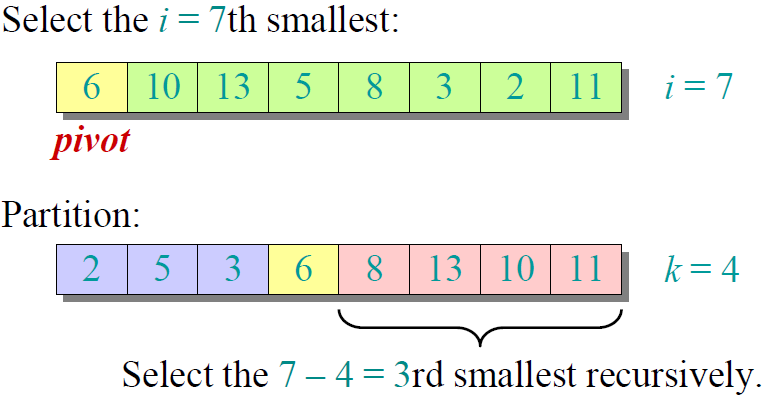
\includegraphics[width=\textwidth]{9.2}
		\caption{}
		\label{fig:9.2}
	\end{figure}\answer{\begin{algorithm}[H]
			\caption{Statistical Order to find the Smallest Element in Linear Time}\label{alg:orderstat}
			\begin{algorithmic}[1]
			\Function{OrderStat}{$A$, $p$, $q$, $i$}\Comment{Initial call: \Call{OrderStat}{$A$, $1$, $n$, $i$}}
				\State $k \gets$ \Call{Partition}{A, p, q}\Comment{$O($size $A$ from $p\rightarrow q)$}
				\If{$i = k$}
					\State \Return $A[k]$
				\ElsIf{$i < k$}
					\State \Return \Call{OrderStat}{$A$, $p$, $k-1$, $i$}
				\Else\Comment{$i > k$}
					\State \Return \Call{OrderStat}{$A$, $k+1$, $q$, $i-k$}
				\EndIf
			\EndFunction
			\end{algorithmic}
		\end{algorithm} Runtime Analysis: \begin{equation*}
		\begin{aligned}
			T(\mbox{size of subproblem}) &= T(n)\\
										 &= O(n) + T\left(\mbox{size of subproblem: } \frac{n}{2} \rightarrow n-1 \right)\\
			T(1) &= O(1)\\
			\mbox{Master method}: T(n) &= aT\left( \frac{n}{b} \right) + f(n)\\
			a &= 1\\
			b &= 2\\
			f(n) &= n^{\log_{2}(1)}=0\\
				 &= 1\\
			\Theta(f(n)) = \Theta(n)
		\end{aligned}
		\end{equation*} Worst case: \begin{equation*}
		\begin{aligned}
			T(n) &= T(n-1) + O(1)\\
				 &= O\left( \frac{n(n-1)}{2} \right)\\
				 &= O\left( n^{2} \right)\\
		\end{aligned}
		\end{equation*}}
	
	\item What is the worst case running time if you find the $i$th smallest element?\\Is there an algorithm to find the $i$th smallest element that runs in linear time in the worst case?\begin{algorithm}[H]
		\caption{Select Smallest Element in Linear Time}\label{alg:select}
		\begin{algorithmic}[1]
		\Function{Select}{$i,n$}
			\State Divide the $n$ elements into groups of 5. Find the median of each 5-element group by hand.
			\State Recursively \Call{Select}{} the median $x$ of the $\lfloor \frac{n}{5} \rfloor$ group medians to be the pivot.
			\State Partition around the pivot $x$. Let $k=$\Call{rank}{$k$}.
			\If{$i = k$}
				\State \Return $x$
			\ElsIf{$i < k$}
				\State Recursively \Call{Select}{} the $i$th smallest element in the lower part
			\Else
				\State Recursively \Call{Select}{} the $(i-k)$th smallest element in the upper part
			\EndIf
		\EndFunction
		\end{algorithmic}
	\end{algorithm}
	\begin{table}[H]
	    \centering
		\label{tab:figs}
		\begin{tabular}{cc}
			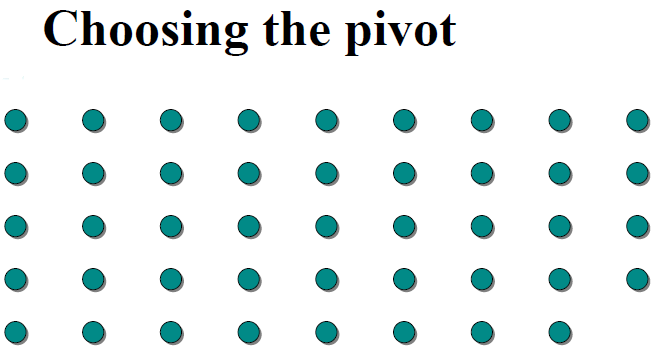
\includegraphics[width=0.45\textwidth,height=0.22\paperheight]{9.3} & 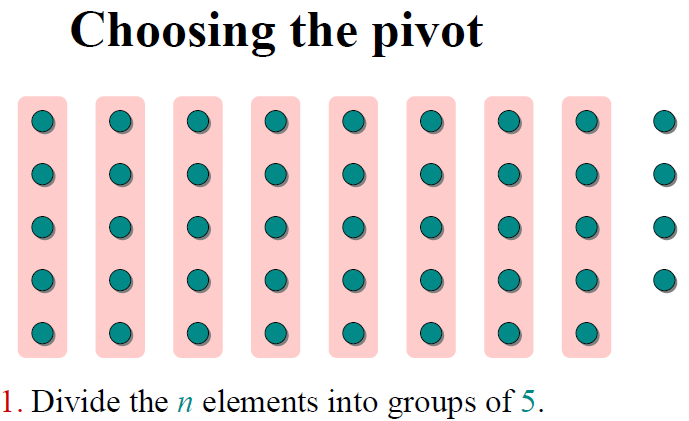
\includegraphics[width=0.45\textwidth,height=0.22\paperheight]{9.4}\\
			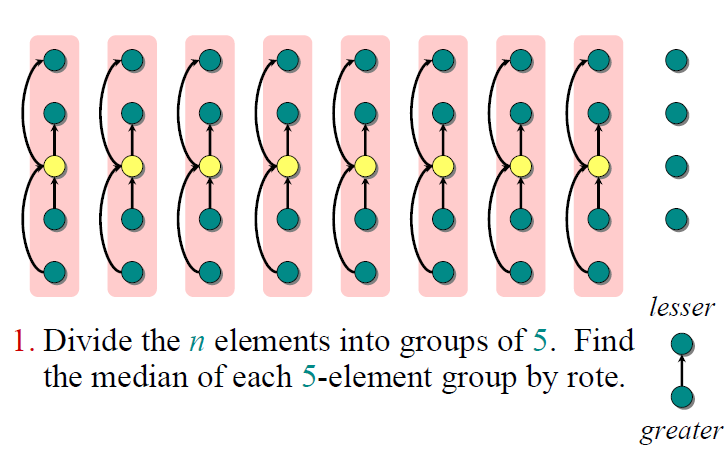
\includegraphics[width=0.45\textwidth,height=0.22\paperheight]{9.5} & 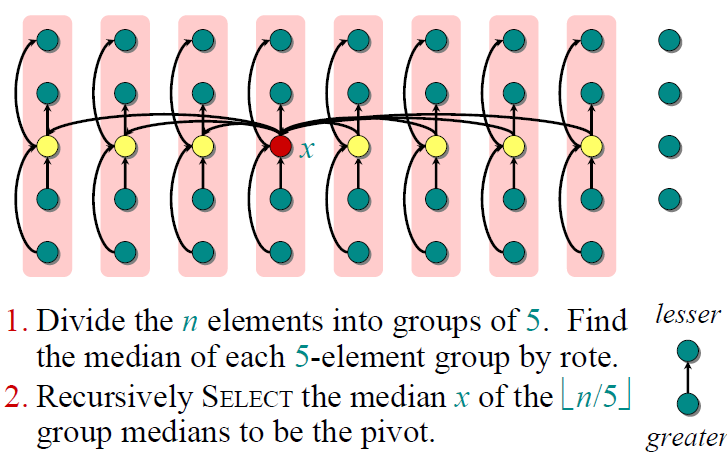
\includegraphics[width=0.45\textwidth,height=0.22\paperheight]{9.6}\\
			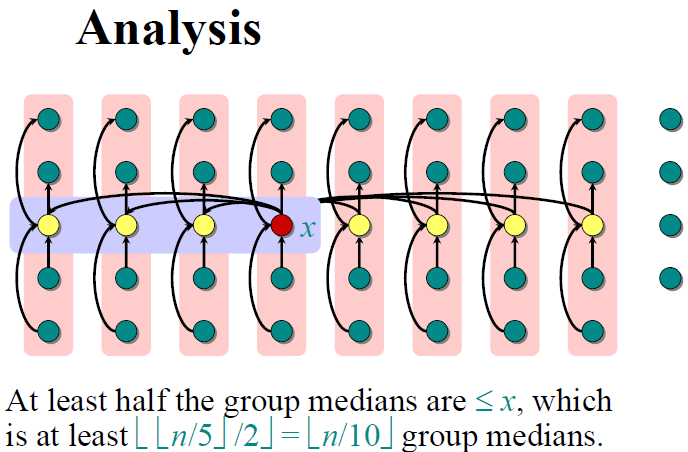
\includegraphics[width=0.45\textwidth,height=0.22\paperheight]{9.7} & 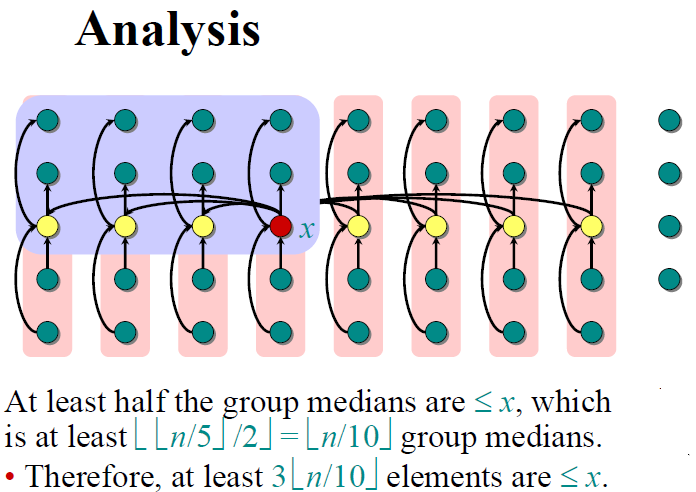
\includegraphics[width=0.45\textwidth,height=0.22\paperheight]{9.8}\\
			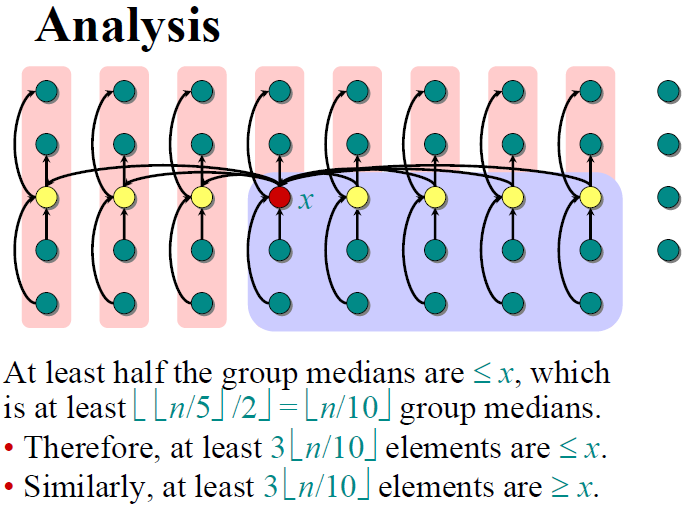
\includegraphics[width=0.45\textwidth,height=0.22\paperheight]{9.9} & 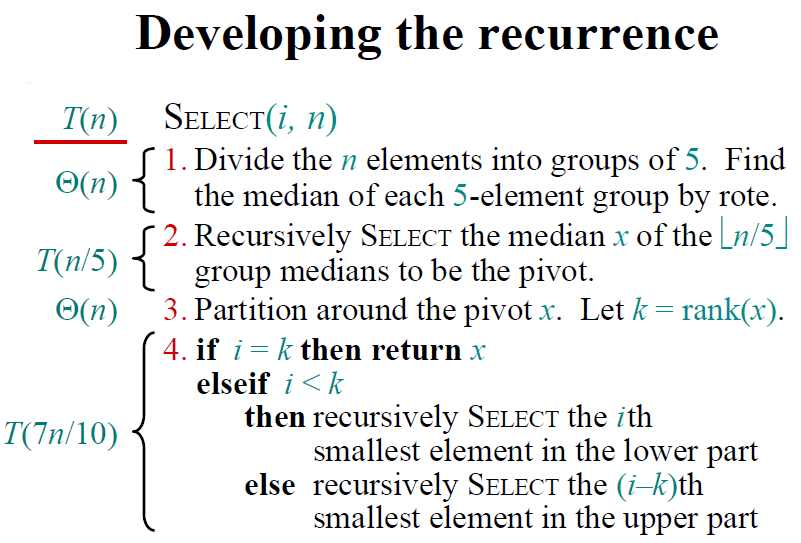
\includegraphics[width=0.45\textwidth,height=0.22\paperheight]{9.developing-the-recurrence}\\
		\end{tabular}
	\end{table}
	\subsection{Solving the recurrence}\label{subsec:solving-the-recurrence}
	\textcolor{recgreen}{\textbf{Substitution:} $T(n) \leq cn$\begin{equation*}
	\begin{aligned}
		T(n) &= T\left( \frac{1}{5}n \right) + T\left( \frac{7}{10} \right) + \Theta(n)\\
		T(n) &\leq \frac{1}{5}cn + \frac{7}{10}cn + \Theta(n)\\
			 &= \frac{9}{10}cn + \Theta(n)\\
			 &= cn - \left( \frac{1}{10}cn - \Theta(n) \right)\\
			 &\leq cn
	\end{aligned}
	\end{equation*}} \answer{if \textcolor{recgreen}{$c$} is chosen large enough to handle the \textcolor{recgreen}{$\Theta(n)$}.}\\\\ In practice, this algorithm runs slowly, because the constant in front of $n$ is large.\\\\Would we use this approach to find the median to partition around in Quicksort, and achieve in worst-case $\Theta(n\log n)$ time? \answer{\textbf{No}, too many calls to $O(cn)$ \hyperref[alg:select]{Select} with a big $c$. We can do this if we need to find the median once or a couple of times, but not inside of Partition.}
\end{enumerate}

%</Lecture-Activity-9>

\end{document}